%This is an example for a chapter, additional chapter can be added in the skeleton-thesis
%To generate the final document run latex, build and quick build commands on the skeleton-thesis file not this one.
%This is chapter 2, the default skeleton thesis expects 2 chapters
\chapter{Findings}
\label{sec:evaluation}

To evaluate the impact of removing permissions on applications, seven common permissions (Table~\ref{tbl:results}) were selected based on their potential threat to the user's security and privacy.  For each permission, 100 applications that declare the permission in their manifests were randomly downloaded.  These applications are from the official Google Play Market as well as other markets in the US, China, and Europe.

\begin{table*}[t]
\centering
\tiny
\begin{tabular}{|l|c|c|c|c|}
\hline
& \# Apps & \# Fatal & \multicolumn{2}{|c|}{\texttt{SecurityException}} \\ \cline{4-5}
Data Set & Run & Exceptions & \# Exceptions & \# Apps Throwing Exceptions\\ \hline 
{\bfseries \ttfamily WRITE\_SMS} Original & 95 & 528 & 1 & 1 \\ \hline
{\bfseries \ttfamily WRITE\_SMS} Removed & 91 & 555 & 1 & 1 \\ \hline
{\bfseries \ttfamily ACCESS\_FINE\_LOCATION} Original & 99 & 623 & 0 & 0 \\ \hline
{\bfseries \ttfamily ACCESS\_FINE\_LOCATION} Removed & 99 & 616 & 18 & 13 \\ \hline					
{\bfseries \ttfamily CAMERA} Original & 97 & 1206 & 0 & 0 \\ \hline
{\bfseries \ttfamily CAMERA} Removed & 97 & 1158 & 0 & 0 \\ \hline
{\bfseries \ttfamily RECORD\_AUDIO} Original & 93 & 700 & 0 & 0 \\ \hline
{\bfseries \ttfamily RECORD\_AUDIO} Removed & 92 & 659 & 0 & 0 \\ \hline
{\bfseries \ttfamily READ\_CALENDAR} Original & 91 & 581 & 0 & 0 \\ \hline 
{\bfseries \ttfamily READ\_CALENDAR} Removed & 91 & 643 & 8 & 6 \\ \hline
{\bfseries \ttfamily READ\_CONTACTS} Original & 96 & 633 & 0 & 0 \\ \hline
{\bfseries \ttfamily READ\_CONTACTS} Removed & 96 & 561 & 40 & 20 \\ \hline
{\bfseries \ttfamily INTERNET} Original & 95 & 191 & 13 & 3 \\ \hline
{\bfseries \ttfamily INTERNET} Removed & 95 & 234 & 13 & 3 \\ \hline
\end{tabular}
\caption{Results of Random UI Introspection}
\label{tbl:results}
\end{table*}


A small portion (less than 3\%) of the applications contained manifests with unusual control characters that APKTool would not process (eg. 0x04), and were discarded.  Additionally, 2\% of the applications caused the emulator to crash and were not able to be tested. \toolname\ installed and tested the remaining ones as described in Section~\ref{sec:method}. 

\toolname\ detects application crashes and their causes from the emulator's logs.  When an application does not have a permission required by an API call, the Android framework will typically throw a \texttt{SecurityException} and the application will then crash unless it catches the exception.  An application may crash due to other reasons as noted by the fatal exception column in (Table~\ref{tbl:results}).  For example, bugs in the application, or when \toolname\ executes an activity that is not meant to be executed by the user.  An additional possibility is that a library acting on the application's behalf receives the \texttt{SecurityException}, and returns the proper error condition, such as a null pointer. Applications that do no check for this kind of error state may crash with other types of exceptions such as \texttt{NullPointerException}.  Since it is not possible to determine the true causes of these exceptions without extensive static analysis of each application, this study focuses on \texttt{SecurityExceptions}, which indicate under-permission.  Among all the crashes, 5.8\% were due to a \texttt{SecurityException}.  The seven permissions are examined separately below.

\paragraph{\bfseries \ttfamily INTERNET}
The cause of the \texttt{SecurityExceptions} was ascertained by examining the logs and screen shots.  The exceptions generated both before and after permission removal were the result of a change in the permissions system in Android 4.2, which requires a new permission, \texttt{WRITE\_APN\_SETTINGS}, for the API calls the applications performed.  This is technically under-permission, but was not caused by removing existing permissions.  In the remainder of our samples, ad libraries were the sole reason for an application's request for the \texttt{INTERNET} permission.  All the versions of the \textit{AdMob} libraries that we examined fail gracefully when the INTERNET permission is removed.  For example,  one version of \textit{AdMob} displays a message to the user as seen in Figure~\ref{fig:removing}. 

\begin{figure}[t]
\centerline{\resizebox{0.4\linewidth}{!}{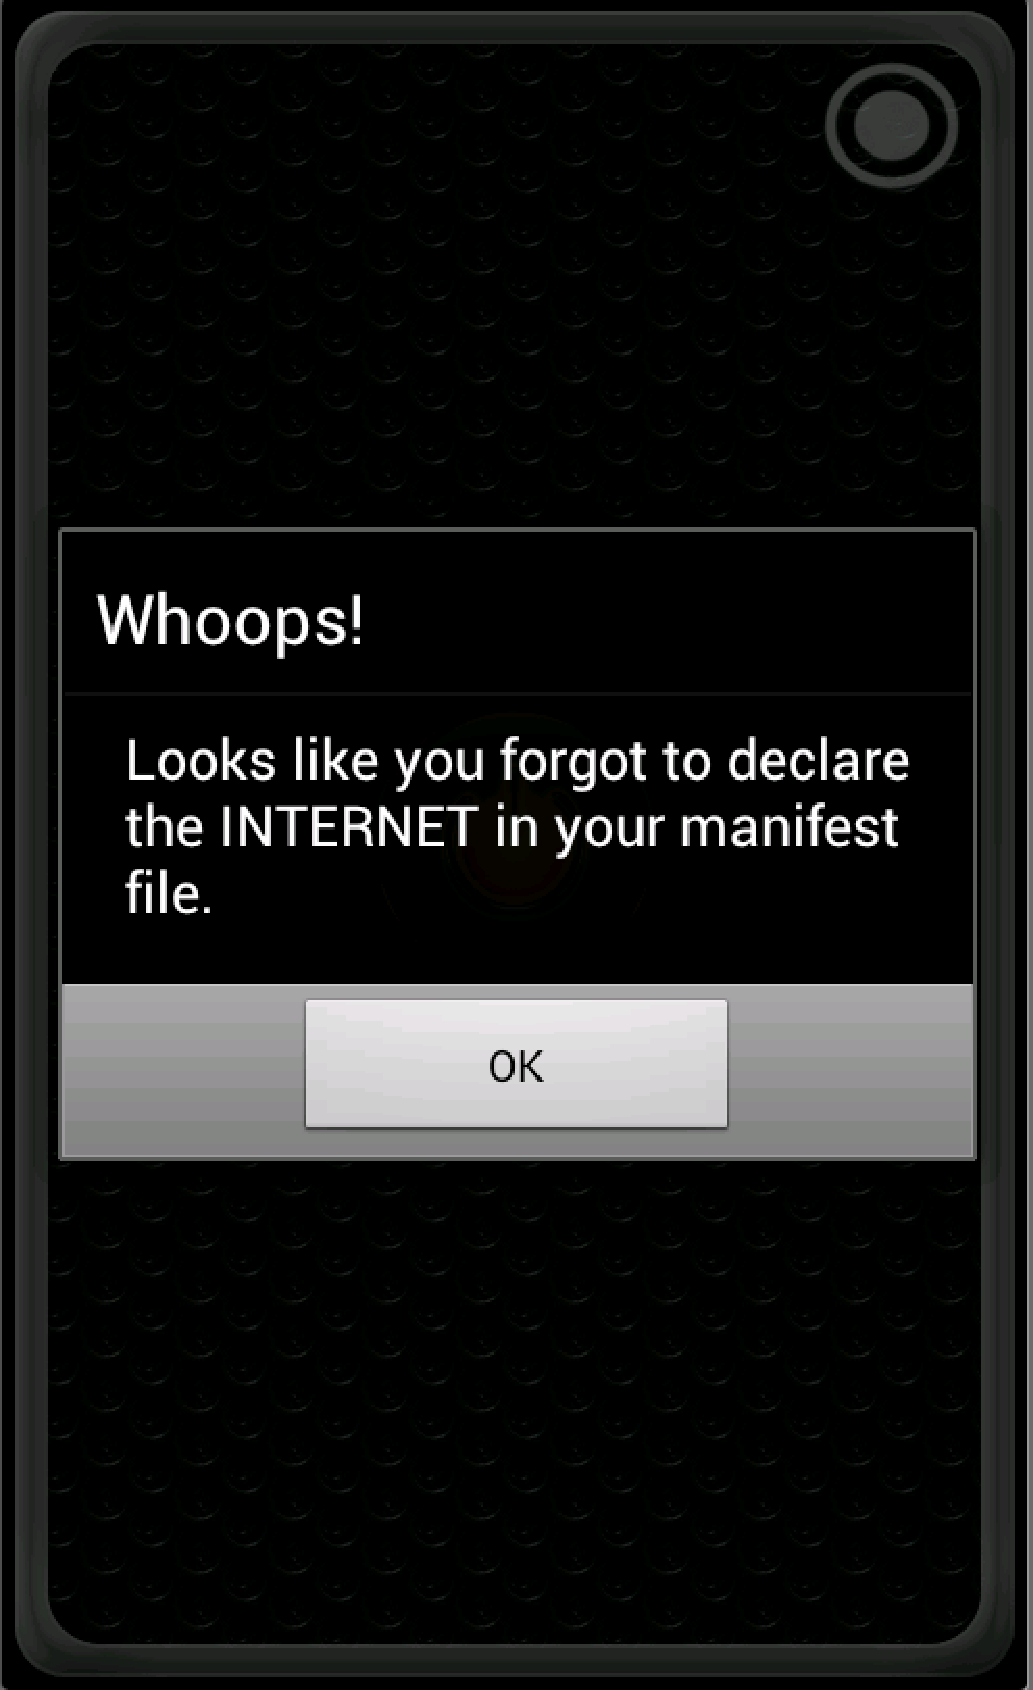
\includegraphics{figure2}}}
\caption{Admob displays a message when the \texttt{INTERNET} permission is removed.}
\label{fig:removing}
\end{figure}

In light of this, a copy of a popular third-party Android web browser was attained and its \texttt{INTERNET} permission removed using \toolname. When executed, the application terminated with a \texttt{SecurityException} related the applications request for DNS information. With further investigation it was determined that the application calls the \texttt{java.net} functions directly causing a \texttt{SecurityException} to be generated and the standard crash screen to be displayed (see Figure~\ref{fig:crash}).

\begin{figure}[t]
\centerline{\resizebox{0.4\linewidth}{!}{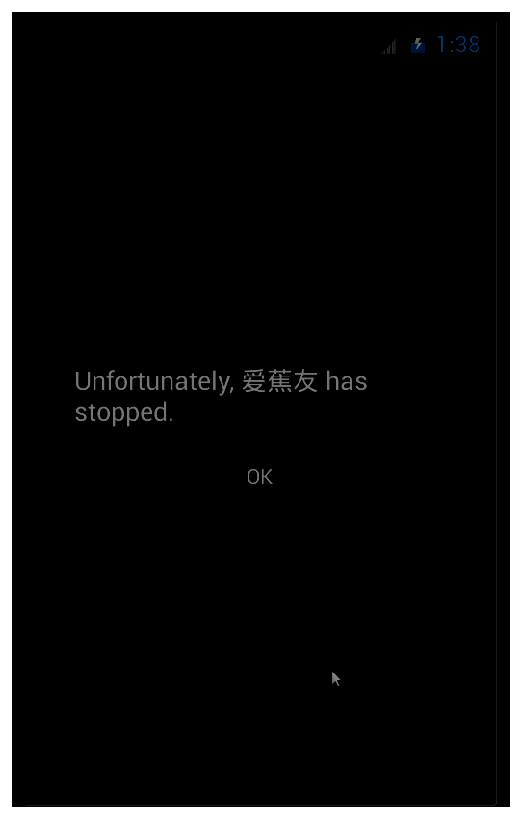
\includegraphics{figure3}}}
\caption{App crashes due to \texttt{SecurityException} when the \texttt{INTERNET} permission is removed.}
\label{fig:crash}
\end{figure}

\paragraph{{\bfseries \ttfamily CAMERA} and {\bfseries \ttfamily RECORD\_AUDIO}}
In the case of \texttt{CAMERA} and \texttt{RECORD\_AUDIO}, both functionalities have a service that proxies application requests.  If the relevant permissions are removed, they will behave as if no camera or microphone is present.  Therefore, no \texttt{SecurityExceptions} were observed when these permissions were removed.

\paragraph{{\bfseries \ttfamily READ\_CONTACTS} and {\bfseries \ttfamily READ\_CALENDAR}}
Manual investigation determined that, when removing \texttt{READ\_CONTACTS}, a \texttt{SecurityException} was only being recieved in cases where the API call to read the contacts was actually occurring. While the presence of some other helper library that catches exceptions cannot completely rule out, in every case that was manually examined, the \texttt{SecurityException} was only occurring when the automated testing specifically activated a UI element or activity's startup code that made a request to the Provider URI, \texttt{content://com.android.contacts/}. 

The removal of \texttt{READ\_CALENDAR} results in similar behavior. Apps attempting to access the Provider URI, \texttt{content://com.android.calendar/}, generate security exceptions in all cases we have examined. 

\paragraph{\bfseries \ttfamily WRITE\_SMS}
The \texttt{WRITE\_SMS} permission also uses a Provider URI, \texttt{content://mms-sms/}; however, no \texttt{SecurityExceptions} resulting from permission removal were observed.  The one that was observed in both test cases was a result of the missing permission, \texttt{WRITE\_APN\_SETTINGS}, that was discussed earlier.  The lack of \texttt{SecurityExceptions} is likely due to the relative depth of writes to this URI within the application, which makes it more difficult to trigger.  Any unauthorized Provider URI access produces the standard crash screen (Figure~\ref{fig:crash}). 

\paragraph{\bfseries \ttfamily ACCESS\_FINE\_LOCATION}
The fine-grained location permission, \texttt{ACCESS\_FINE\_LOCATION}, is a special case. It is one of a few permissions in Android that is a nested permission. Many API calls will operate in the presence of either fine or coarse location permissions but prefer fine; if fine is removed it will fall back to coarse grain location. This results in few \texttt{SecurityExceptions} (\textasciitilde13\%), since they will only occur in cases where the GPS hardware is explicitly being used.

